\documentclass[hidelinks,11pt,twoside,a4paper]{report}



\usepackage[portuguese]{babel}
\usepackage[utf8]{inputenc}
\usepackage{hyperref}
\usepackage{amsmath}
\usepackage{amssymb}
\usepackage{float}
\usepackage{xspace}% used by \sigla
\usepackage[printonlyused]{acronym}
\usepackage{listings}
\usepackage{url}
\usepackage{indentfirst}
\usepackage{color,soul}
\usepackage{booktabs}
\usepackage{graphicx}
\newcommand{\hlc}[2][yellow]{ {\sethlcolor{#1} \hl{#2}} }


\renewcommand{\baselinestretch}{1.2}
\setcounter{tocdepth}{3}

\begin{document}

%definoções
\def\titulo{Realidade Virtual - Uma visão.}
\def\data{12/11/2017}
\def\autores{Tomás Martins, Daniel Lopes}
\def\autorescontactos{(89286) tomasfilipe7@ua.pt, (87881) daniel.vnl@ua.pt}
\def\departamentoacr{DETI}
\def\departamento{Departamento de Eletrónica, Telecomunicações e Informática}
\def\empresa{Universidade de Aveiro}
\def\logotipo{imagens/ua.pdf}



%página de titulo
\begin{titlepage}

\begin{figure}[H]
\centering

\includegraphics[scale=1]{imagens/ua.pdf} 
\end{figure}

%
\centering
{\Large \empresa}
%

%
\vspace{5mm}
%
\centering
{\Large \data}


\begin{center}
%
\vspace*{50mm}
%
{\Huge \titulo}\\ 
%
\vspace{10mm}
%

%
\vspace{20mm}
%
{\LARGE \autores}\\ 
%
\vspace{30mm}
%
\begin{figure}[h]
\center

\end{figure}
%
\vspace{30mm}
\end{center}
%

\end{titlepage}


% pagina de titulo secundária
\title
{
{\Huge\textbf{\titulo}}\\
{\Large \departamentoacr\\ \departamento\\ \empresa}	
}
%
\author{%
    \autores \\
    \autorescontactos
}
%
\date{\data}
%
\maketitle
\begin{titlepage}\end{titlepage}

%indice em numeração romana
\pagenumbering{roman}
\tableofcontents

\cleardoublepage
\chapter*{Acrónimos}
\begin{acronym}[XXXXXXXX]
	\acro{RV}{\textit{Realidade Virtual}}
	\acro{HMD}{\textit{Head Mounted Display}}
\end{acronym}	

\cleardoublepage
\pagenumbering{arabic}
\renewcommand{\abstractname}{Resumo}
\begin{abstract}
\paragraph{}
Atualmente já todos ouvimos falar de Realidade Virtual, mas nem todos sabem em que consiste.Esta é uma tecnologia de interface avançada que proporciona ao utilizador a sensação de estar num ambiente alternativo.

É uma tecnologia que pode ser imersiva ou não imersiva, que tem vindo cada vez mais a evoluir, desde a invenção do Estereoscópio no séc. XIX.Após uma evolução bastante atribulada, passando por diversas máquinas de todo o estilo e tamanho, está agora num patamar de tecnologia bastante avançada graças á evolução dos computadores e dos smartphones.

Inicialmente foi concebida para a área do entertenimento, tanto para filmes como para jogos, já tendo sido alargada para diversas áreas tais como:Medicina, onde é usada tanto para o tratamento de novos cirurgiões, como para cura de fobias, como para Odontologia; é usado também na área Militar com o propósito de um treino militar em ambientes mais seguros; Por fim é utilizada também em Simuladores, para simular aviões e comboios, pois acidentes com estes mesmos transportes resultam em grandes tragédias.

Para toda esta tecnologia funcionar cada vez melhor e dar ao utilizar uma experiencia cada vez mais imersiva, serve-se de muitos tipos de equipamentos, tais como: HMDs, luvas, fatos...

No entanto, apesar de todas estas vantagens, acaba por ser bastante dispendiosa.É também uma tecnologia muito avançada, o que significa que é preciso computadores potentes para a suportar, e acima de tudo pode causar dependência ou certos acidentes, pois as pessoas não vão estar cientes do verdadeiro meio que as rodeia.



\end{abstract}

%capitulos
\cleardoublepage
\pagenumbering{arabic}
\chapter{Introdução}

Vivemos num mundo com a tecnologia a avançar a cada dia que passa a um ritmo assustadoramente alto e todos os dias são inventados e desenvolvidos novos hardwares e softwares.Nesta última década, um grande termo de tecnologia que se tem ouvido falar é a "Realidade Virtual", também conhecida como "Realidade Aumentada".Desde a medicina aos videojogos,entre outras áreas que irão ser exploradas posteriormente neste relatório, esta tem se provado bastante util e eficaz e cada vez mais acessível aos consumidores.

Quando ouvimos falar de Realidade Virtual, automaticamente o nosso cérebro conduz-nos para uma imagem de tecnologia moderna com equipamentos e softwares de última geração que nos levam a navegar num mundo completamente alternativo.No entanto a Realidade Virtual é bem mais antiga e mais complexa do que essa nossa imagem.\\

\section{Organização do Trabalho}

A partir deste Capítulo, este trabalho está organizado da seguinte forma:\\

\textbf{•  }\textbf{Capítulo 2 - Mas então o que é a realidade virtual?}.\\

\textbf{•  }\textbf{Capítulo 3 - HMD}:.\\

\textbf{•  }\textbf{Capítulo 4 - História}: .\\

\textbf{•  }\textbf{Capítulo 5 - Realidade Virtual - Áreas de aplicação}: .\\

\textbf{•  }\textbf{Capítulo 6 - Caracteristicas da Realidade Virtual}: .\\

\textbf{•  }\textbf{Capítulo 7 - Equipamentos}: .\\

\textbf{•  }\textbf{Capítulo 8 - Vantagens e Desvantages}: .\\

\textbf{•  }\textbf{Capítulo 9 - Realidade Virtual: o Presente e o Futuro}: .\\

\textbf{•  }\textbf{Conclusão}: .\\
	




\cleardoublepage
\chapter{\bf Mas então o que é a realidade virtual?}
\paragraph{}
\section{Formação léxica da palavra.}
\paragraph{}
Podemos facilmente decompor Realidade Virtual em duas simples palavras: "Realidade" e "Virtual".
\begin{enumerate}
\item[\bf{Virtual: }]Virtual é algo "que tem a força de exercer-se, mas que não se exerce", "suscetível a realizar-se";"é algo feito ou simulado através de meios eletrónicos"\cite{7}.
\item[\bf{Realidade: }]Realidade é a existência efetiva de algo;
\end{enumerate}

Podemos então concluir que o termo "Realidade Virtual" significa que é possivel criar ou simular algo que realmente existe mas que apesar de tudo não é verdadeiro.
\section{Conceito}
\paragraph{}
	Toda a realidade que experienciamos, é apenas uma combinação de todos os nossos sentidos(ex:audição,olfato,etc...), e esta tecnologia serve-se desses mesmos sentidos para gerar um ambiente e uma interação não real de maneira a enganar a perceção do utilizador sobre o meio onde se encontra.
	\begin{figure}
	\center
	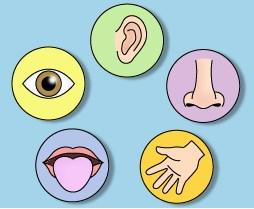
\includegraphics[scale=0.4]{imagens/sentidos.jpg}
	\caption{5 sentidos principais do corpo humano.\cite{1} }
	\end{figure}
	
	A Realidade Virtual é então uma "forma de visualizar,manipular, explorar,interagir e modificar dados complexos através do computador"\cite{8} que interfere com os nossos sentidos de maneira a criar uma sensação de falsa realidade.
	
	"Atualmente esta tecnologia é conseguida através de equipamentos tecnológicos tal como capacetes , monitores e luvas, que servem para ampliar a estimulação dos sentidos" \cite{9}
	"No entanto o nosso cérebro não é fácil de enganar, visto que os nossos sentidos e o nosso cérebro evoluiram de maneira a que todo o nosso redor esteja perfeitamente sincronizada" o que faz com que ao minimo erro nesta tecnologia, nós conseguimos diferenciar o real do imaginário.Nasce então assim a politica dos 3 Is na Realidade Virtual.Para tirarmos proveito desta tecnologia ao máximo,a mesma tem de obedecer a 3 simples passos:
	\begin{enumerate}
	\item[1]- \textbf{Imersão:}Qualquer software e hardware de realidade virtual tem de ser imersivo, servindo-se dos sentidos do ser humano para o fazer.
	\item[2]- \textbf{Interação:} maneira a captar a atenção do nosso cérebro, tem de existir uma interação entre homem-máquina.Cada vez mais são inventados novos géneros de hardware sofisticados que permitam esta interação ser cada vez mais real.
	\item[3]- \textbf{Imaginação:} Um programa que usufrui desta tecnologia tem obrigatoriamente de estimular a imaginação do utilizador.Se isso não acontecer, não é possivel criar a sensação de uma realidade alternativa.
	\end{enumerate}

	
	\begin{figure}
	\center
	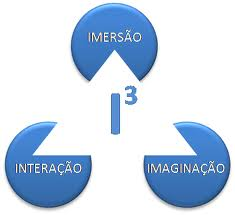
\includegraphics[scale=0.5]{imagens/3is.jpg}
	\caption{Representação da trilogia dos 3 I's \cite{2}}
	\end{figure}


\cleardoublepage
\chapter{HMD}
		\paragraph{} 
Uma parte significativa dos softwares de realidade aumenta requerem um uso de HMDs e a sua evolução está diretamente relacionada com a evolução da realidade virtual.\paragraph{}
 Mas o que é um HMD? \paragraph*{}
 HMD é um aparelho usado na cabeça, cujo objetivo é transmitir informação de forma visual através de um ecrã posicionado em frente a um ou ambos os olhos.O primeiro foi inventado por Morton Heilig(também inventor do Sensorama), e consistia num capacete com um ecrã que reproduzia um filme com uma visão estereoscópica em 3D , no entanto não inclua qualquer tipo de sensor de movimento ou interação com o usuário. 
 \begin{figure}
 \center
 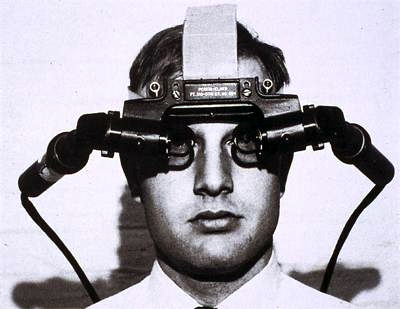
\includegraphics[scale=0.5]{imagens/HMD.jpg}
 \caption{Primeiro HMD, também conhecido como Sword of Damocles. \cite{3}}
 \end{figure}
\thispagestyle{empty}






\cleardoublepage
\chapter{História}
\label{cap.historia}
\paragraph{}
\section{História}
	A cada dia que passa, esta tecnologia avança cada vez mais, e atualmente já é possivel retirarmos proveito de diversas maneiras deste conceito de realidade virtual.Esta foi um objeto de estudo durante vários anos, e foi progredindo de forma lenta e pouco regular, sendo a sua grande expansão, apenas na última década.
	\subsection{Estereoscópio - 1838}
		\paragraph{}
Ao que tudo indica, o pioneiro desta tecnologia foi Sir Charles Wheatstone que inventou o Estereoscópio, um aparelho de análise de diversas imagens em diferentes perspectivas com o objetivo de oferecer a ilusão de uma vista tridimensional.
			\begin{figure}
				\center
%				\includegraphics[scale=0.3]{imagens/Estereoscópio.jpg}
				\caption{Estereoscópio \cite{4}}
			\end{figure}
	\subsection{\textit{Pygmalion’s Spectacles - 1935}}
	\paragraph{}
Escrito por Stanley G. Weinbaum a 1935,  \textit{Pygmalion's Spectacles} é uma pequena história onde o protagonista conhece um professor que inventa uns óculos que permitiam a uma pessoa sentir-se dentro do filme que estão a ver, algo muito parecido com o que no futuro se tornou a realidade virtual.
	\subsection{Sensorama - 1955}
 \paragraph{}
 Foi então em 1955 que o pioneiro nesta tecnologia, Morton Heilig, visionou, e mais tarde em 1962 acabou por o desenvolver, o primeiro projeto de realidade virtual como nós a conhecemos .
 
O Sensorama é uma máquina que tem como propósito a reprodução de filmes acompanhados dos mais diversos efeitos sensoriais de maneira a criar imersão ao utilizador.Servia-se de uma visão de imagens estereoscopicas em 3D , combinado com um movimento do corpo,cheiros e vento de acordo com o ambiente da imagem e sons em \textit{stereo} durante a reprodução do filme(Uma versão mais primitiva do que se intitula nos dias de hoje de: Cinema 4D).

Apesar de todo o sucesso, Heilig não foi capaz de obter apoio financeiro para as suas patentes, o que obrigou o término deste projeto.
	\begin{figure}
	\center
	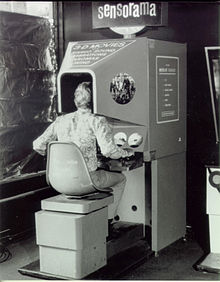
\includegraphics[scale=0.5]{imagens/Sensorama.jpg}
	\caption{Sensorama. \cite{5}}
	\end{figure}
	\subsection{Headsight - 1961}
	\paragraph{}
Headsight foi o primeiro HMD a integrar sensores de movimento."É constituido por um ecrã para cada olho e por um sensor de movimentos conectado a uma câmera por um circuito fechado.Ao contrário do que pode parecer, nao foi desenvolvida com propósitos de Realidade Virtual, mas para efeitos militares,cujo objetivo seria visualizar os perigos de certas situações."\cite{10}
	
	\subsection{Ultimate Display - 1965 / Sword of Damocles - 1968}
\paragraph{}
Seguindo a ideia por trás do Sensorama, Ivan Sutherland escreve o artigo: \textit{The Ultimate Display}, que revolucionou o pensamento da época e acabou por impulsionar a ideia de Realidade Virtual.Sutherland disserta sobre a ideia da evolução tecnológica e do seu potencial e limites,referindo que "um computador não tem de se limitar ás leis da fisica tal como nós"\cite{11}, admitindo por fim, que o \textit{"auge da tecnologia(\textbf{ Ultimate Display}) seria um computador capaz de alterar toda a matéria numa sala , incluindo gerar cadeiras que seriam possiveis de se sentar , algemas que conseguiriam prender e balas que poderiam ser fatais.Com a programação certa, este dispositivo poderia ser literalmente o País das Maravilhas em que a Alice entrou "}\cite{11}.

Poucos anos mais tarde , este mesmo senhor desenvolveu um protótipo bastante rudimentar este artigo, ao qual intitulou de "\textit{Sword of Damocles}".Este dispositivo ainda ficava muito aquém, tanto na interface de usuário como no grafismo da aplicação.Semelhante ao Sensorama,o sistema de reprodução era feito entre o computador e um ecrã estereoscópico.Continha um sensor de movimento no HMD, o que juntamente com o estereoscópio, que permitia o ecrã ajustar-se á posição da pessoa.

A primeira aplicação a ser desenvolvida para este aparelho, era um cubo suspenso por um fio, em frente ao utilizador e era composto por uma série de diversos hardwares.Esta ideia foi inspirada na história do nome do próprio aparelho:"\textit{Sword of Damocles}", que nos conta uma breve história sobre Damocles, um homem do povo ao qual foi dada a proposta que poderia ser rei por um dia, mas teria uma espada presa por apenas um fio de cabelo de um cavalo por cima do seu trono. 
\begin{figure}
\center
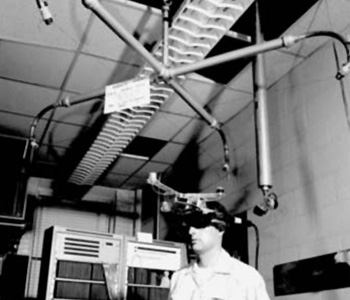
\includegraphics[scale=0.4]{imagens/SOD.jpg}
\caption{Sword of Damocles -  Era uma máquina intimidante e pouco prática. \cite{6}}
\end{figure}
	\subsection{Realidade Artificial - 1969}
\paragraph{}
Myron Kruegere , um artista de realidade virtual, conduziu uma série de testes na tentativa bem sucedida de criar um mundo que interagisse e respondesse ás ações do usuário.Através desta tecnologia , era possivel as pessoas comunicarem umas com as outras num ambiente gerado por um computador.
	\subsection{O nascimento do nome - 1987}
\paragraph{}
Apesar de toda esta tecnologia, ainda não existia um termo que associasse e unisse toda esta tecnologia.Jaron Lanier apelidou então, em 1987, este campo de "Realidade Virtual".
	
A sua empresa começou então a desenvolver equipamentos para esta área, tais como luvas e óculos.
	\subsection{Consumo Público - 1991}
\paragraph{}
Foi na década de oitenta e noventa que a Realidade Virtual começou a ganhar força, no entanto ainda estava bastante inacessivel para uma utilização caseira.Chega-nos consequentemente o lançamento de máquinas de jogos arcade de RV pelo TVG. Os jogadores utilizariam um par de óculos e disfrutavam do jogo em tempo real, e alguns desses jogos até chegavam a estar conectados numa rede para incluir um modo multi jogador.
\begin{figure}
\center
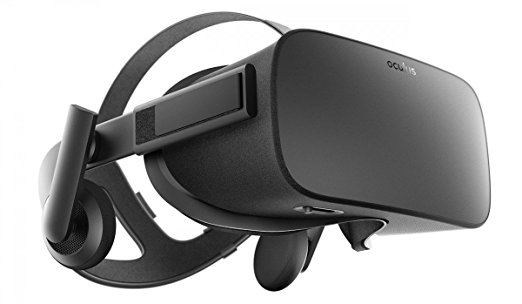
\includegraphics[scale=0.3]{imagens/OR.jpg}
\caption{Oculus Rift}
\end{figure}
\subsection{Inicio das consolas VR - 1993}
\paragraph{}
Em 1993, a SEGA lançou um novo produto de óculos de RV para a sua consola SEGA Genesis.Estes óculos disfrutavam de sensor de movimento, som em \textit{stereo} e um ecrã em LCD. Infelizmente, devido a problemas técnicos e apesar de terem sido lançados 4 jogos para esta plataforma, a mesma nunca chegou a passar de uma fase de protótipo.
\subsection{Realidade Virtual nos dias de hoje}
\paragraph{}
Ninguém pode negar que o crescimento da Realidade Virtual tem sido exponencial, e começou o seu grande desenvolvimento no séc. XXI.A tecnologia dos computadores é cada vez mais avançada e a acessibilidade dos produtos ao consumidor é cada vez mais facil.A evolução dos smartphones contribuiu bastante também para a explosão da Realidade Virtual, pois permite-nos ter dispositivos portáteis com bastante capacidade e potência, nunca deixando de ser leves e de boa mobilidade.Enquanto isso, a industria dos video-jogos continua o seu desenvolvimento, sempre na liderança da utilização desta tecnologia.

Muitas empresas estão a começar a investir nesta área, tais como a Google que desenvolve headsets controlados por smarthphones, a Samsung que implementa novas funções de realidade virtual a cada produto Galaxy que lançam, e até mesmo o Facebook, o que começou como uma rede social , chegou mesmo a comprar os direitos dos Oculus Rift, um dos HMDs mais populares da atual geração, competindo com grandes nomes da área de entertenimento como a Valve, Microsoft e Sony.






\cleardoublepage
\chapter{Realidade Virtual - Áreas de aplicação}

Após uma apresentação do conceito e da história da \acl{RV}, este capítulo vem apresentar um conjunto de aplicações ligadas atualmente à \acl{RV}\footnote{Apenas alguns exemplos de áreas de aplicação.}.
 
\section{Medicina}

\subsection{Treino Médico}
Esta área de aplicação permite que os pacientes tenham uma melhor interação e compreensão sobre o corpo humano, construindo e/ou reaprendendo novas capacidades que serão posteriormente aplicadas em situações reais. Todas estas novas habilidades são realizadas em ambiente virtual, garantindo assim a máxima segurança dos pacientes.
Em ambiente de ensino, podemos dar o exemplo da Odontologia, onde os alunos podem trabalhar por um conjunto de dentes em \emph{3D} e executar uma série procedimentos clínicos próprios, como por exemplo, uma broca virtual.

\subsection{Paramédicos}
Na área dos Paramédicos e outras atividades equivalentes, a \acl{RV} é também utilizada em treinos de medicina. Com isto, os futuros médicos aprendem a desenvolver novas capacidades de socorro rápido sem colocar ninguém em risco. 

\subsection{Tratamento de Fobias}	
No tratamento de fobias a \acl{RV} também tem a sua aplicação. Por exemplo, tratar pacientes que tenham medo de andar de avião, de estar em alturas ou estar na presença de determinados animais. O paciente sabe que está num ambiente totalmente seguro, mas o cérebro confunde-se e reage como se da realidade se tratasse. Com isto torna-se muito mais simples para o médico ajudar o paciente e também poderá aumentar ou diminuir a dificuldade do tratamento.

\begin{figure}[h]
\center
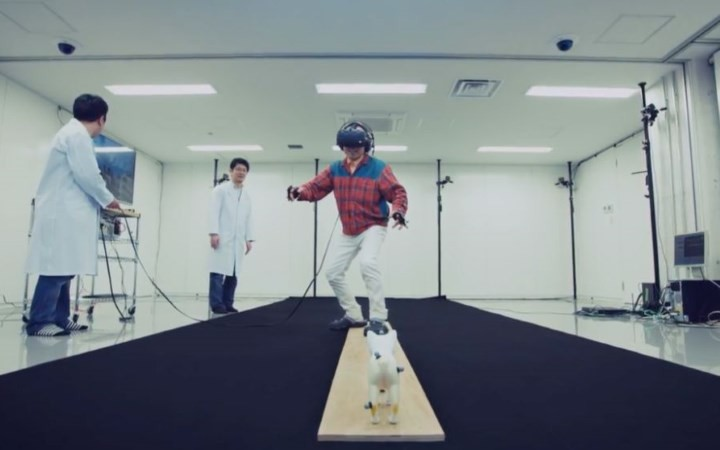
\includegraphics[scale=0.4]{imagens/RV_tratamento_fobia.jpg}
\caption{Exemplo do tratamento da fobia de alturas. Simulação em RV \cite{RV_fobia_1}}
\end{figure}

\section{Jogos}
Na década de 80 e 90 várias foram as empresas que tiveram a tentativa de começar com a \acl{RV} mas sem sucesso, isto porque não haviam recursos computacionais suficientes para que tal fosse possível. As empresas estavam mais focadas em tentar relacionar a Realidade Virtual com jogos, temos o exemplo, já mencionado noutro capitulo, da SEGA que em 1993 anunciou os \emph{Sega VR headsets}, mas devido a problemas a empresa desistiu do produto, nunca tendo chegado ao mercado.

Em 2009 a \emph{Palmer Luckey}, na garagem dos seus pais criou o primeiro protótipo do \emph{Oculus Rift}. Foi este o inicio dos óculos virtuais \cite{RV_fundador}.

Mais tarde, a playstation lançou a \emph{Playstation VR}. A \emph{Playstation VR} utiliza o comando da \emph{PS4} e um comando semelhante ao da \emph{Nintendo Wii}, que reconhece os movimentos do usuário e assim a experiência torna-se muito mais real.

A \emph{HTC} também juntou-se a este mercado em parceria com a \emph{Valve} anunciando o \emph{HTC Vive}.
este equipamento exige que o utilizador adquira um computador potente e que tenha mais espaço disponível. Até agora o \emph{HTV Vive} é o único que tem comandos especialmente desenvolvidos para uma maior interação.


\section{Simuladores}
\subsection{Simulador de Comboio}

Os Simuladores de Comboios permitem emular exatamente o comportamento do comboio, tendo como objetivo ser uma ferramenta prática e confiável para o treino dos maquinistas.

Existem diversos elementos que constituem este sistema, desde a escolha da locomotiva, travões, potência, modelo etc. O sistema é capaz de simular a condução normal de um comboio e para além disso também é capaz de reproduzir várias condições atmosféricas. O sistema também permite a configuração do comboio, simulando degradações no mesmo de forma a avaliar a capacidade do maquinista \cite{RV_comboio}.


\subsection{Simulador de Voo}

Do mesmo modo que os simuladores de comboios, os simuladores de voo são utilizados para o treino de pilotos. Estes têm como objetivo atribuir qualificações aos tripulantes técnicos. Somente nestes equipamentos é possível treinar e simular diversas situações com grande realismo, isto sem por em risco a vida das pessoas.
O uso deste tipo de simuladores de voo no âmbito de treinar, proporciona uma enorme economia em combustível. Como consequência, o custo das formações será mais reduzido assim como o impacto no ambiente, porque não haverá queima de combustível, reduzindo assim os gases carbónicos que são emitidos \cite{RV_aviao}.

\begin{figure}[h]
\center
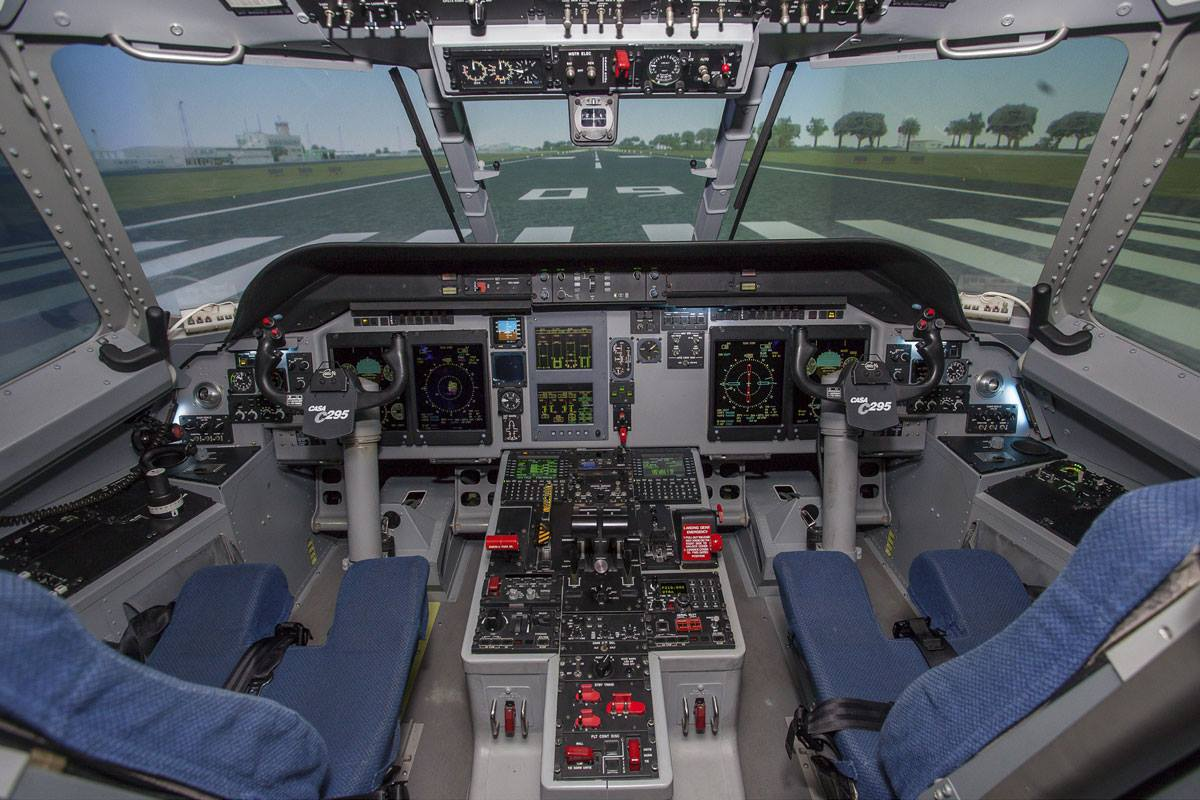
\includegraphics[scale=0.2]{imagens/RV_simulador_voo.jpg}
\caption{Exemplo de um simulador de voo. \cite{RV_sim_voo}}
\end{figure}

\section{Área militar}

Na industria militar também a realidade virtual é aplicada em simuladores, sendo o seu principal objetivo treinar militares num ambiente seguro sem qualquer tipo de consequências. 

A Força Aérea, o Exército e a Marinha usam por exemplo, os simuladores de voo, no âmbito de treinar os seus pilotos. Alguns exemplos desta simulação é abastecer em caso de emergência ou voar num campo de batalha ou até mesmo como coordenar a sustentação no ar com ajudar de operações terrestres \cite{RV_militar}.







\cleardoublepage
\chapter{Características da Realidade Virtual}

\section{Imersiva}

Realidade imersiva, significa tal como o nome diz, uma realidade em que o seu utilizador sente-se imerso. É uma sensação em que o seu utilizador experimenta sensações quase reais dentro do ambiente virtual, podendo este interagir com os seus elementos. 
Os exemplos mais comuns da realidade imersiva são por exemplo simuladores de voo, capacetes, oculus rift, luvas virtuais, fato virtual, Icaros \cite{RV_inter}. 

\section{Não imersiva}

Realidade não imersiva, é basicamente o oposto do que foi dito na realidade imersiva em que o seu usuário tem a sensação de que está num ambiente real. A realidade não imersiva não consiste na sensação de inclusão experimentada pelo usuário, pois ele não se sente dentro do ambiente virtual, é esta realidade que a maior parte das pessoas estão acostumadas a experimentar, por exemplo, quando um usuário está a jogar jogos num computador comum, ou seja, esteja a visualizar o jogo no ecrã e a interagir nele com o rato e teclado, ou até mesmo um comando, a isto é que definido como sendo a realidade não imersiva \cite{RV_inter}.

\section{Interativa}
Já foi dito o que significava realidade imersiva, mas o que significa a realidade interativa? 
A realidade interativa é aquela em que o seu usuário pode interagir com os elementos dentro da realidade virtual, por exemplo, um usuário que esteja num ambiente simulado pode manipular objetos virtuais e o equipamento mais comum para que isso seja possível é o uso de luvas virtuais \cite{RV_inter}.









\cleardoublepage
\chapter{Equipamentos}

\section{Oculus Rift}

O equipamento é constituído por dois ecrãs OLED, um para cada olho e tem uma resolução de 1080x1200 cada, tem um ângulo de visão de 270 graus, isto cobre praticamente o campo de visão do usuário dando-lhe a máxima experiência do mundo virtual. É também constituído por três giroscópios que capta os movimentos da cabeça do utilizador.

O primeiro protótipo dos Oculus Rift, foi criado em 2009 por Palmer Luckey, este mesmo mais tarde criou uma empresa chamada Oculus que mais tarde em 2014 foi comprada pela empresa Facebook Inc.

Para usar os Oculus Rift é recomendado um computador com capacidades acima das mínimas, pois a realidade virtual requer um pouco das capacidades do computador.

\vspace{5mm}
\begin{figure}[h]
\center
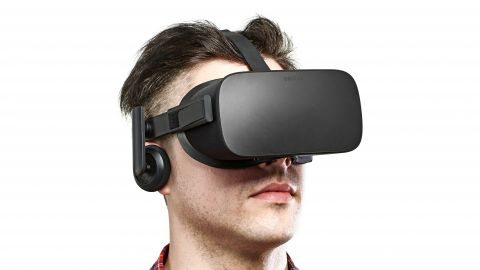
\includegraphics[scale=0.6]{imagens/RV_OR.jpg}
\caption{Exemplo de Oculus Rift. \cite{RV_OR}}
\end{figure}
\vspace{10mm}

\section{Luvas Virtuais}
Luvas virtuais são dispositivos que através de sensores, detetam e medem as flexões e abduções dos dedos, as luvas virtuais na maioria dos casos não são usadas em aplicações sem o apoio de outros equipamentos, ou seja, normalmente pode-se usar juntamente com um fato virtual, um capacete virtual ou os oculus rift. É com a presença destes três equipamentos que obtemos a intitulada realidade virtual.

As luvas virtuais também são usadas no âmbito da medicina (discutida no capitulo anterior). Está a ser testado este equipamento nesta área principalmente para simular operações delicadas, naquelas em que pode não pode haver contacto entre o médico e o paciente pelo risco de morte.


\begin{figure}[h]
\center
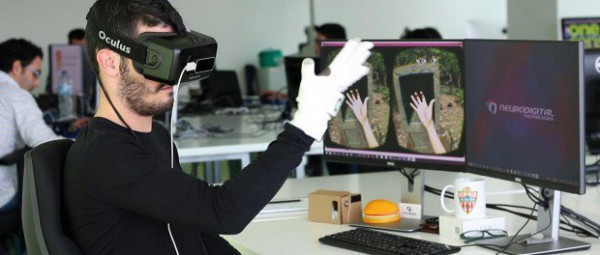
\includegraphics[scale=0.6]{imagens/RV_luvas.jpg}
\caption{Luvas virtuais. \cite{RV_luvas}}
\end{figure}


\section{Icaros}

O Icaros é um simulador que tem como objetivo criar uma sensação de que a pessoa está a flutuar. Utilizando os óculos da realidade virtual juntamente com um aplicativo desenvolvido pelo próprio fabricante, é criado um ambiente praticamente imersivo.

Com ICAROS podemos simular diversas situações desde saltar de uma montanha com paraquedas ou saltar de um avião.

Mas o objetivo do Icaros não é só simular situações de voo, o Icaros também é capaz de simular por exemplo uma moto em alta velocidade, pois o sistema também possui capacidade para tal. No fundo o Icaros é parecido com uma prancha suspensa e possui apoios para os braços e pernas, também é um aparelho para fazer exercício físico, com ele usuário pode treinar diversos grupos musculares, tudo isto dentro da realidade virtual, o usuário poderá fazer exercícios, como subir escadas ou andar de bicicleta. 



\begin{figure}[h]
\center
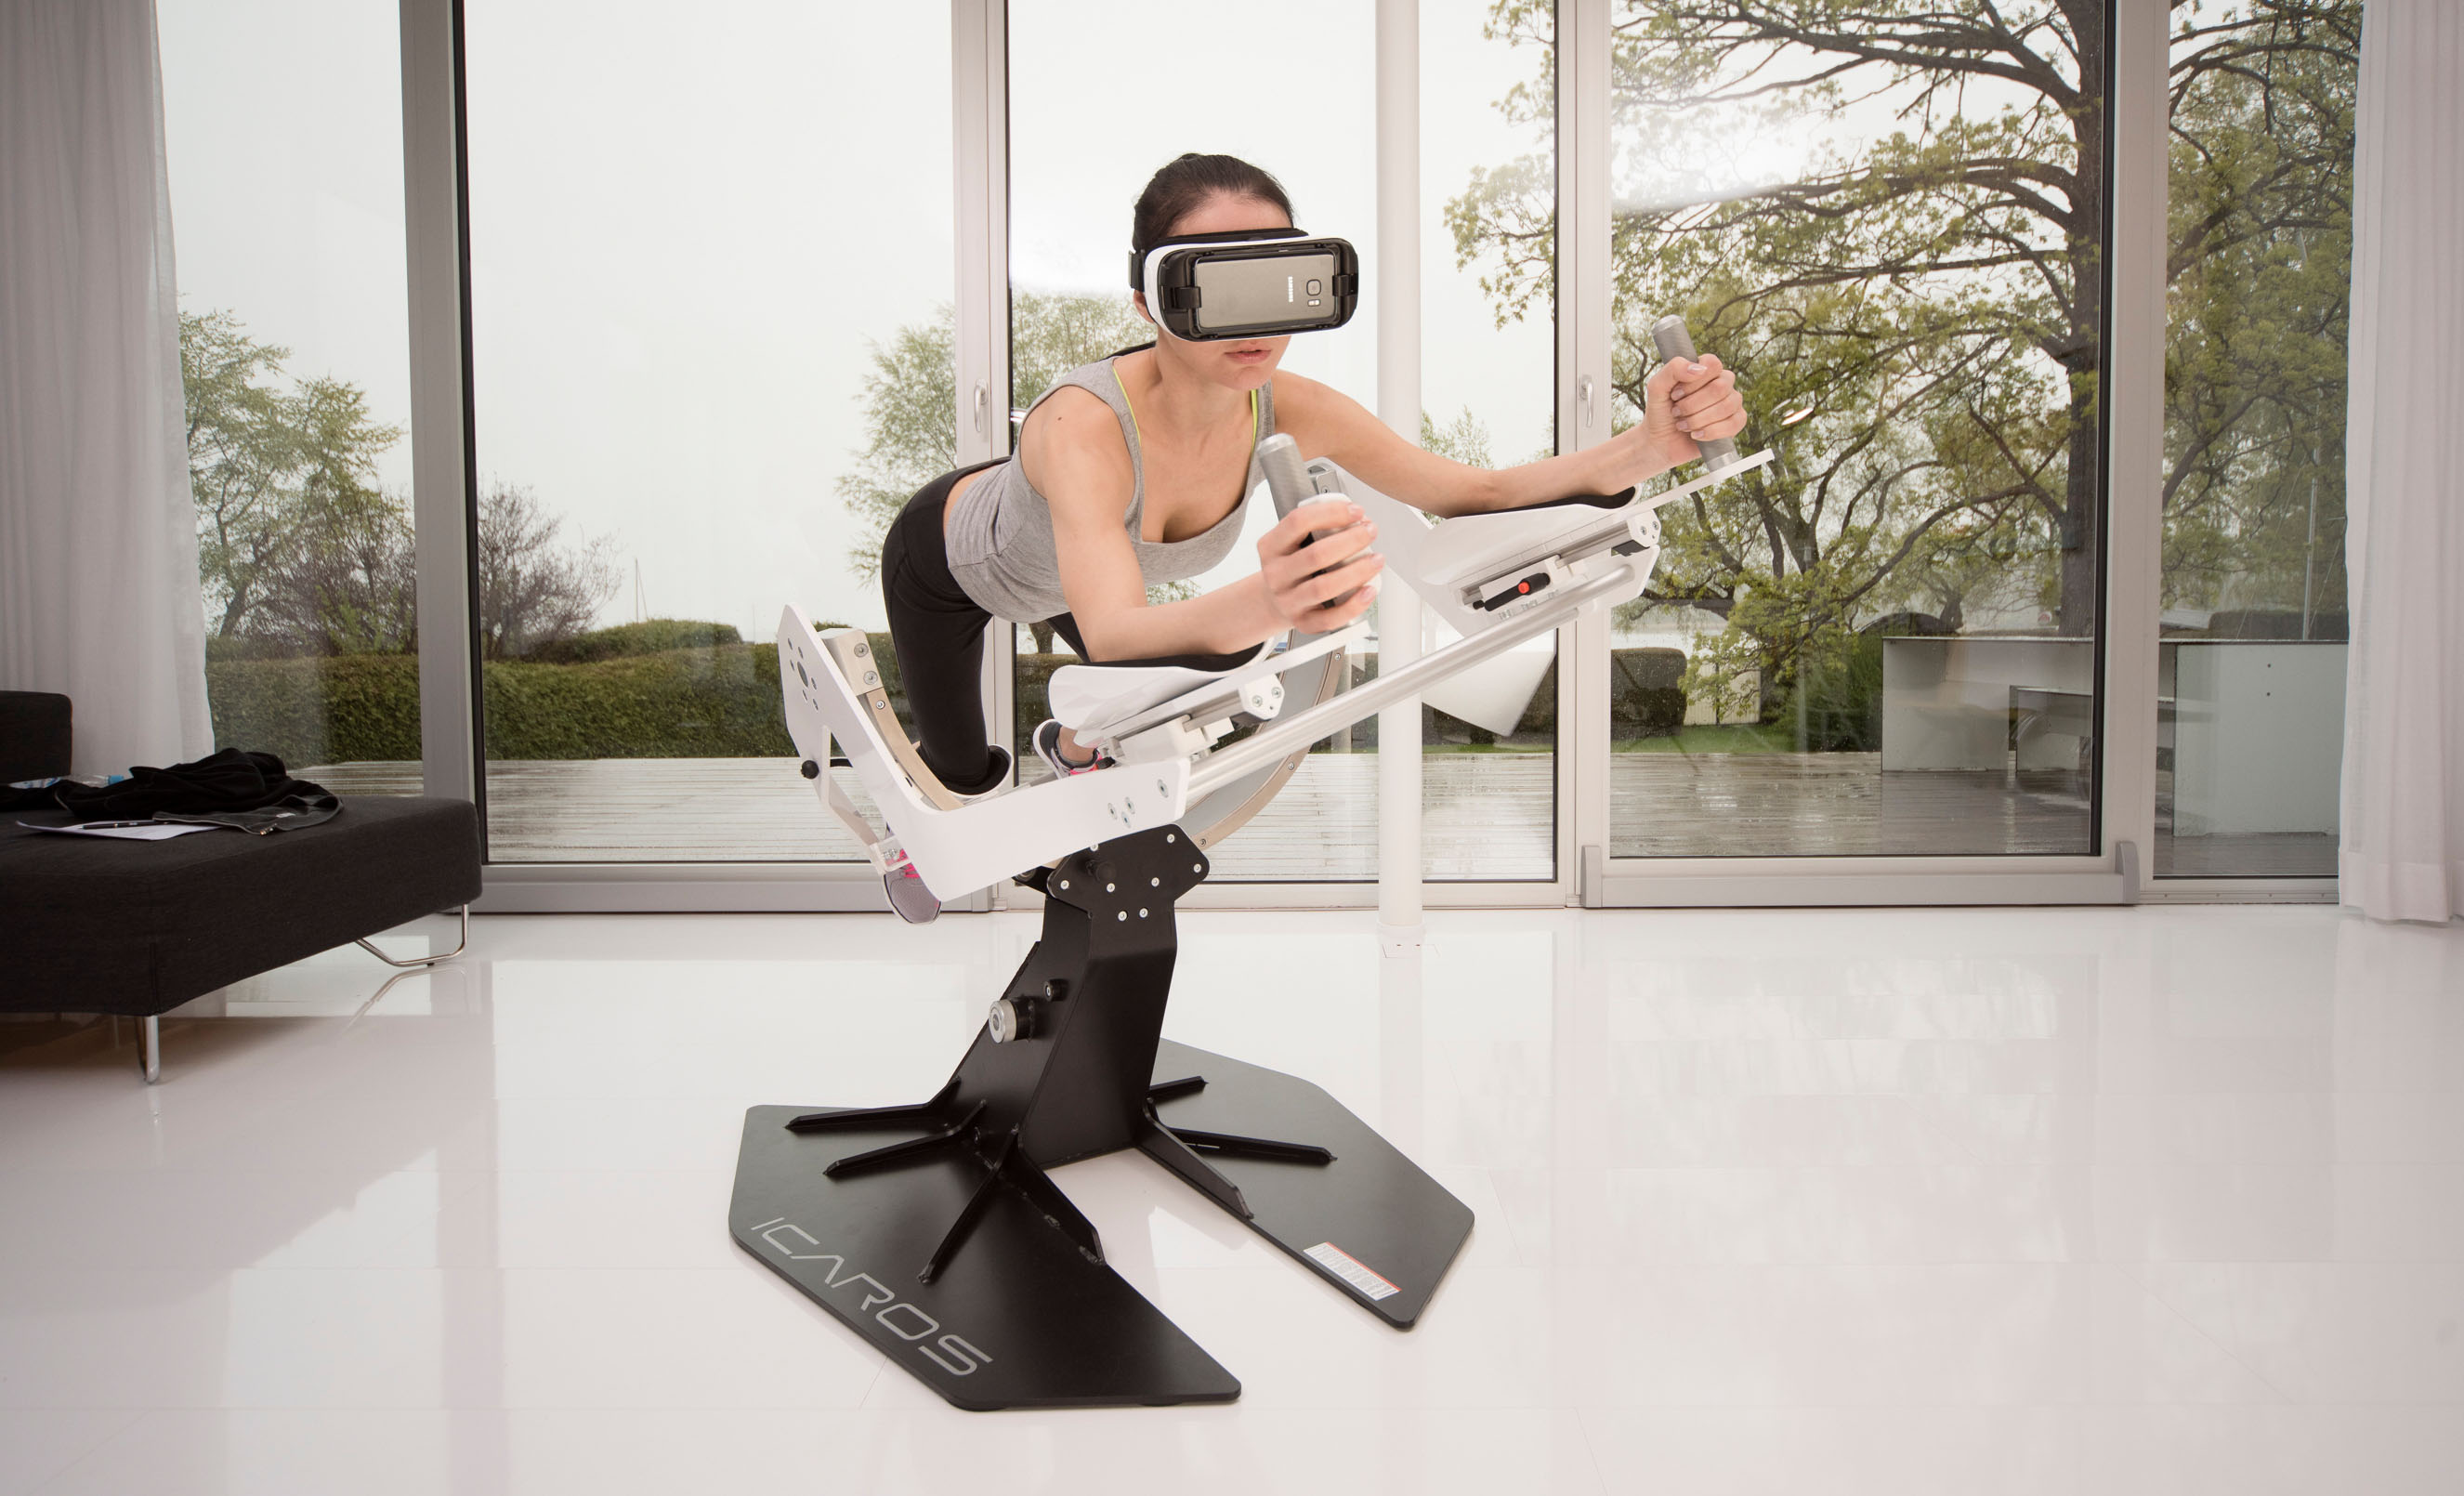
\includegraphics[scale=0.6]{imagens/RV_icaros.jpg}
\caption{Icaros. \cite{RV_icaros}}
\end{figure}


\section{Fato virtual}

Fato virtual Hardlight VR Suit é especialmente desenvolvido para quem é amante de jogos virtuais.

Este fato funciona juntamente com outros equipamentos VR, mas também com jogos de computador comuns.

Este equipamento cobre o tronco e braços por completo e por cada toque que o personagem do jogo sentir o seu usuário no mundo real também sentirá através dos seus 16 sensores espalhados pelo fato que emitem vibrações.


\begin{figure}[H]
\center
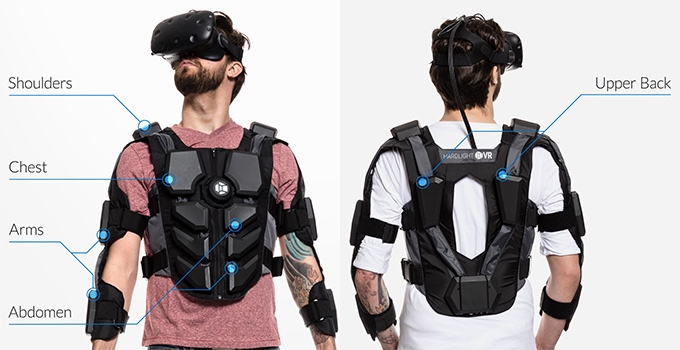
\includegraphics[scale=0.5]{imagens/RV_fato.jpg}
\caption{Fato virtual. \cite{RV_fato}}
\end{figure}





\cleardoublepage
\chapter{Vantagens e Desvantagens}

\section{Vantagens}

A Realidade Virtual  veio facilitar em grande parte processos outrora não dominados pelo ser humano, reduzindo imenso os custos assim como a perda de vidas humanas. 
Através da simulação podemos controlar diversos equipamentos à distância. 
Possibilita a execução de várias simulações de forma a treinar profissionais sem qualquer tipo de perigo real, com baixos custos de manutenção. No caso de simuladores de voo por exemplo as emissões de gases para a atmosfera não existem, o que contribui para redução do flagelo do efeito de estufa.
Na medicina a realidade virtual também pode ajudar muito mais eficazmente no tratamento de fobias, treino de operações, etc.


\section{Desvantagens}

Uma vez que esta tecnologia está a dar os seus primeiros passos na história da humanidade, a sua produção ainda acarreta custos elevados, como por exemplo o seu custo. O preço de um automóvel novo é equivalente ao custo dos equipamentos da Realidade Virtual, mas atenção não estamos a falar de um simples equipamento como o Oculus Rift, mas sim, da realidade totalmente imersiva. 

Tal como acima mencionado a Realidade Virtual é uma tecnologia recente e posto isso ainda não está desenvolvida de maneira que possa ser executada num tradicional computador pessoal pois a capacidade do seu processamento ainda é muito elevada o que requer poderosos computadores.

E como o perigo certamente não é uma vantagem, vale a pena numerar alguns perigos desta nova tecnologia. Um dos perigos é quando os usuários estiverem a utilizar por exemplo os Oculus Rift certamente não terão noção do que se passa à sua volta, isso tornará o usuário completamente vulnerável ao mundo real, se este estiver em locais públicos poderá facilmente ser roubado ou algo pior, se estiver dentro de casa também existirá o perigo pois o usuário não verá os objetos que existem á sua volta no mundo real, estará submerso num mundo onde os objetos reais não existem e isso poderá levar a certos danos físicos se no caso estiver a explorar o mundo virtual.






\cleardoublepage
\chapter{Realidade Virtual - O Presente e o Futuro}


É claro que ainda existem muitas pessoas que não conhecem o termo de Realidade Virtual e imaginam que ainda é algo que poderá estar num futuro ainda um pouco distante, mas a realidade hoje em dia já é outra, a Realidade Virtual já forma um mercado que movimenta 5,2 bilhões de dólares por ano. Jogos com precisão e realismo impressionantes, filmes completamente imersivos num ambiente em 360 graus, concertos onde será possível andar perto do cantor favorito, parques de diversões simulados, visitas a museus mundialmente conhecidos apartir de casa.

A realidade já evolui de tamanha forma e continuará a evoluir, tanto que no futuro poderá ser possível trabalhar em casa, estando ao mesmo tempo no escritório ou fazer uma reunião com outras pessoas. No futuro poderão aparecer as lentes de contacto, com elas poderá ser possivel ajustar a visão, reunir informações sobre a saúde, inserir elementos digitais no campo de visão ou até mesmo criar uma realidade completamente virtual.




	





\cleardoublepage
\chapter{Conclusão}

Nunca a tecnologia avançou tanto como hoje. Uma prova disso é o aparecimento de tecnologias de \acl{RV} mais sofisticadas, sendo algumas delas até mesmo acessíveis ao utilizador comum.
No futuro poderão aparecer as lentes de contacto e com elas poderá ser possivel ajustar a visão, reunir informações sobre a saúde, inserir elementos digitais no campo de visão ou até mesmo criar uma realidade completamente virtual.
Espera-se também que seja possível interagir a nível cerebral com realidades virtuais criadas em poderosos computadores e quem sabe, o ser humano tornar-se uma espécie híbrida.

\cleardoublepage
\chapter{Créditos}

Este trabalho foi realizado no âmbito da Unidade Curricular de \emph{Laboratórios de Informática} e teve colaboração de:\\

\textbf{Daniel Lopes}\\
\textbf{•  }\textbf{Capitulo 1}.\\
\textbf{•  }\textbf{Capitulo 5}.\\
\textbf{•  }\textbf{Capítulo 6}.\\
\textbf{•  }\textbf{Capítulo 7}.\\
\textbf{•  }\textbf{Capítulo 8}.\\
\textbf{•  }\textbf{Capítulo 9}.\\
\textbf{•  }\textbf{Conclusão}.\\


\textbf{Tomás Martins}\\

\textbf{•  }\textbf{Capitulo 1}.\\
\textbf{•  }\textbf{Capítulo 2}.\\
\textbf{•  }\textbf{Capítulo 3}.\\
\textbf{•  }\textbf{Capítulo 4}.\\


Ambos os autores tiveram igual participação na estruturação e organização do documento.


%
% Bibliografia
%
\cleardoublepage
\bibliographystyle{unsrt}
\bibliography{bibliografia}




\end{document}
